% Todo
% - Falar da Caffe
%
%

\documentclass{beamer}
\mode<presentation>{
  %   \usetheme{CambridgeUS}      % or try Darmstadt, Madrid, Warsaw, ...
  \usetheme{Frankfurt}
  %   \definecolor{mygreen}{cmyk}{1,0.11,0.82,0.25}
  %   \definecolor{mygreen}{cmyk}{0.6,0.168,0.168,0.25}
  %   \definecolor{mygreen}{cmyk}{0.4,0.02,0.00,0.31}
  % \definecolor{mygreen}{RGB}{107,172,175}
  \definecolor{mygreen}{RGB}{84,135,138}
  \setbeamercolor{structure}{fg=mygreen}
  \usefonttheme{default}
  \setbeamertemplate{navigation symbols}{}
  %\setbeamertemplate[compatibility=false, numbered]{caption}
  \setbeamertemplate{itemize items}[default]
  \setbeamertemplate{enumerate items}[default]

  \defbeamertemplate*{title page}{customized}[1][]{
  \centering
   \begin{beamercolorbox}[rounded=true,shadow=true,leftskip=1cm,colsep*=.75ex]{title}
   \usebeamerfont{title}\inserttitle\par
    \end{beamercolorbox}
     \par\medskip\medskip\medskip
     \begin{columns}

     \begin{column}{0.6\textwidth}
     \centering{
          \usebeamerfont{author}\insertauthor\par\medskip\medskip
          \usebeamerfont{institute}\insertinstitute\par\medskip\medskip
          \usebeamerfont{date}\insertdate\par
          \medskip \medskip \medskip
          \includegraphics[height=0.8cm]{figuras/cnpqLogo.jpg}
    }
    \end{column}
    \begin{column}{0.3\textwidth}
    \includegraphics[width=\columnwidth]{figuras/brasao_usp_pb}
    \end{column}
    \end{columns}
  }

  \setbeamertemplate{footline}{
    \begin{beamercolorbox}[colsep=1.5pt]{upper separation line foot}
    \end{beamercolorbox}
    \hbox{%
   \begin{beamercolorbox}[wd=0.82\paperwidth, ht=2.5ex, dp=1.125ex, left]{title in head/foot}%
        \usebeamerfont{title in head/foot}\hspace*{2ex}\insertshorttitle
      \end{beamercolorbox}%

      \begin{beamercolorbox}[wd=0.09\paperwidth, ht=2.5ex, dp=1.125ex, center]{title in head/foot}%
        \usebeamerfont{author in head/foot}{\insertshortinstitute }
      \end{beamercolorbox}%
     
      \begin{beamercolorbox}[wd=0.09\paperwidth, ht=2.5ex, dp=1.125ex, right]{title in head/foot}%
        \usebeamerfont{title in head/foot}\insertframenumber/\inserttotalframenumber\hspace*{2ex}
      \end{beamercolorbox}}
    \begin{beamercolorbox}[colsep=1.5pt]{lower separation line foot}
    \end{beamercolorbox}
  }

}

\usepackage{ragged2e}
\usepackage{lipsum}

\makeatletter
\renewcommand{\itemize}[1][]{%
  \beamer@ifempty{#1}{}{\def\beamer@defaultospec{#1}}%
  \ifnum \@itemdepth >2\relax\@toodeep\else
    \advance\@itemdepth\@ne
    \beamer@computepref\@itemdepth% sets \beameritemnestingprefix
    \usebeamerfont{itemize/enumerate \beameritemnestingprefix body}%
    \usebeamercolor[fg]{itemize/enumerate \beameritemnestingprefix body}%
    \usebeamertemplate{itemize/enumerate \beameritemnestingprefix body begin}%
    \list
      {\usebeamertemplate{itemize \beameritemnestingprefix item}}
      {\def\makelabel##1{%
          {%
            \hss\llap{{%
                \usebeamerfont*{itemize \beameritemnestingprefix item}%
                \usebeamercolor[fg]{itemize \beameritemnestingprefix item}##1}}%
          }%
        }%
      }
  \fi%
  \beamer@cramped%
  \justifying% NEW
  %\raggedright% ORIGINAL
  \beamer@firstlineitemizeunskip%
}
\makeatother

\usepackage[compatibility=false]{caption}
\usepackage{subcaption}
\usepackage[brazil]{babel}
\usepackage[utf8x]{inputenc}
\usepackage{setspace}
\usepackage{ragged2e}
\usepackage{graphicx}
\usepackage{amsmath,amsfonts,amssymb}
\usepackage{xcolor}
\usepackage{url}
\usepackage{array}
\usepackage{gensymb}
\usepackage{multicol}
\usepackage[loadonly]{enumitem}
\newlist{arrowlist}{itemize}{1}
\setlist[arrowlist]{label=$\Rightarrow$}
\usepackage{listings}
\newcommand{\fonte}[1]{\caption*{Fonte: #1}}
\newcommand{\fonteminha}{\caption*{Fonte: Elaborado pelo autor.}}

\title[\textbf{Geração de imagens artificiais e extração de características latentes aplicadas à classificação de imagens}]{\textbf{Geração de imagens artificiais e extração de características latentes aplicadas à classificação de imagens}}
\author{Gabriela Salvador Thumé \\ \vspace{4pt}
        \tiny Orientador: Prof. Dr. Moacir Pereira Ponti Junior}
\institute[ICMC/USP]{Instituto de Ciências Matemáticas e de Computação \\
Universidade de São Paulo \\ }
\date{27 de março de 2015}
%%%%%%%%%%%%%%%%%%%%%%%%%%%%%%%%%%%%%%%%%%%%%%%%%%%%%%%%%%%%%%%%%%%%%%%%%%%%%%%
\begin{document}
\setbeamercovered{transparent}
\begin{frame}[plain]
  \maketitle
\end{frame}
%%%%%%%%%%%%%%%%%%%%%%%%%%%%%%%%%%%%%%%%%%%%%%%%%%%%%%%%%%%%%%%%%%%%%%%%%%%%%%%
\begin{frame}[noframenumbering]{Estrutura da Apresentação}
\setstretch{1.2}
\begin{multicols}{2}
  \tableofcontents
\end{multicols}
\end{frame}
%%%%%%%%%%%%%%%%%%%%%%%%%%%%%%%%%%%%%%%%%%%%%%%%%%%%%%%%%%%%%%%%%%%%%%%%%%%%%%%
\AtBeginSection[]{
\begin{frame}<beamer>[noframenumbering]{Estrutura da Apresentação}
\setstretch{1.2}
\begin{multicols}{2}
\tableofcontents[currentsection, sectionstyle=show/shaded,
]
% \tableofcontents[currentsection,currentsubsection, hideothersubsections, 
%     sectionstyle=show/shaded,
% ]
\end{multicols}
\end{frame}
}
%%%%%%%%%%%%%%%%%%%%%%%%%%%%%%%%%%%%%%%%%%%%%%%%%%%%%%%%%%%%%%%%%%%%%%%%%%%%%%%
\section{Introdução}
\begin{frame}{Introdução}
\setstretch{1.2}
\setlength\leftmargini{0em}
\justifying
\begin{itemize}
\item Classificação de imagens;
\pause
\item Algoritmos de aprendizado de máquina;
\item Generalização para classificar novos exemplos;
\pause
\item Conjuntos de características que dificultam a diferenciação entre as classes;
\item Encontrar as características que melhor discriminam as classes.
\end{itemize}
\end{frame}
%-----------------------------------------------------------------------------
\subsection{Motivação}
\begin{frame}[plain]{Motivação}
\begin{figure}
    \includegraphics[height=0.9\textheight]{figuras/flow.png}
    \caption{Etapas Canônicas.}
\end{figure}
\end{frame}
%-----------------------------------------------------------------------------
\begin{frame}{Motivação}
\setstretch{1.2}
\setlength\leftmargini{0em}
\justifying
\begin{itemize}
\item Maior esforço ao operar no espaço de características já obtidas;
\item Transformações do espaço ou sistemas complexos de classificação para lidar com as deficiências das características extraídas;
\item Características que podem ser exploradas além dos métodos clássicos;
\end{itemize}
\end{frame}
%-----------------------------------------------------------------------------
\begin{frame}{Motivação - Características Latentes}
\setlength\leftmargini{0em}
\justifying
\setstretch{1.2}
\begin{itemize}
\item Métodos de processamento e preparação de imagens antes da extração dessas características;
\item Podem revelar características latentes, não visíveis nas imagens originais;
\item Objetivo: encontrar tais características que possam melhor descrever certas classes do problema.
\end{itemize}
\end{frame}
%-----------------------------------------------------------------------------
\begin{frame}{Motivação - Características Latentes}

\renewcommand{\tabcolsep}{0.0cm}
\begin{figure}[htbp]
 \begin{center}
\begin{subfigure}{.15\textwidth}
  \centering
  \includegraphics[width=\linewidth]{\detokenize{figuras/alga_05b.png}}
  \caption{}
\end{subfigure}
\begin{subfigure}{.15\textwidth}
  \centering
  \includegraphics[width=\linewidth]{\detokenize{figuras/alga_05c.png}}
  \caption{}
\end{subfigure}
\begin{subfigure}{.15\textwidth}
  \centering
    \includegraphics[width=\linewidth]{\detokenize{figuras/alga_05d.png}}
  \caption{}
\end{subfigure}
\begin{subfigure}{.15\textwidth}
  \centering
  \includegraphics[width=\linewidth]{\detokenize{figuras/alga_05e.png}}
  \caption{}
\end{subfigure}
\\
\begin{subfigure}{.15\textwidth}
  \centering
  \includegraphics[width=\linewidth]{\detokenize{figuras/alga_05ba.png}}
  \caption{}
\end{subfigure}
\begin{subfigure}{.15\textwidth}
  \centering
  \includegraphics[width=\linewidth]{\detokenize{figuras/alga_05ca.png}}
  \caption{}
\end{subfigure}
\begin{subfigure}{.15\textwidth}
  \centering
  \includegraphics[width=\linewidth]{\detokenize{figuras/alga_05da.png}}
  \caption{}
\end{subfigure}
\begin{subfigure}{.15\textwidth}
  \centering
  \includegraphics[width=\linewidth]{\detokenize{figuras/alga_05ea.png}}
  \caption{}
\end{subfigure}
\\
\begin{subfigure}{.15\textwidth}
  \centering
  \includegraphics[width=\linewidth]{\detokenize{figuras/alga_05bb.png}}
  \caption{}
\end{subfigure}
\begin{subfigure}{.15\textwidth}
  \centering
  \includegraphics[width=\linewidth]{\detokenize{figuras/alga_05cb.png}}
  \caption{}
\end{subfigure}
\begin{subfigure}{.15\textwidth}
  \centering
  \includegraphics[width=\linewidth]{\detokenize{figuras/alga_05db.png}}
  \caption{}
\end{subfigure}
\begin{subfigure}{.15\textwidth}
  \centering
  \includegraphics[width=\linewidth]{\detokenize{figuras/alga_05eb.png}}
  \caption{}
\end{subfigure}
  \caption{Características latentes de algas verdes.}
%{Características latentes de algas verdes. A primeira imagem (a) é uma imagem original segmentada de alga. As próximas colunas são imagens resultantes da deconvolução da imagem (coluna 2), filtragem Gaussiana (coluna 3) e filtragem Gaussiana seletiva (coluna 4). A primeira linha mostra versões diferentes de imagens de algas, a segunda linha exibe imagens resultantes da diferença de Gaussianas, e a terceira linha demonstra imagens binárias obtidas por limiarização das imagens contidas na segunda linha). \textit{Fonte:~Elaborado pelo autor.}}
 \end{center}
\end{figure}
\renewcommand{\tabcolsep}{0.25cm}
\end{frame}
%-----------------------------------------------------------------------------
\begin{frame}{Motivação - Desbalanceamento de classes}
\setlength\leftmargini{0em}
\justifying
\setstretch{1.2}
  \begin{itemize}
    \item Diferença entre o número de exemplos disponíveis;
    \item Obstáculo;
    \item Métodos de transformação do espaço de características e de classificação assumem que as classes da base estão balanceados;
    \item Objetivo: geração de imagens artificiais. %para rebalancear a base, possivelmente melhorando o modelo criado para a classificação
  \end{itemize}
\end{frame}
%-----------------------------------------------------------------------------
\begin{frame}{Proposta da Pesquisa}
 \setstretch{1.5}
\begin{block}{}
\justifying
    Melhorar a classificação de imagens, utilizando métodos de processamento com foco na \textbf{extração de características latentes} e no \textbf{rebalanceamento de classes.}
\end{block}
\end{frame}
%-----------------------------------------------------------------------------
\subsection{Contextualização}
\begin{frame}{Contextualização}
\setlength\leftmargini{0em}
\justifying
 \setstretch{1.2}
  \begin{itemize}
\justifying
    \item Grupo de pesquisa em Visualização, Imagens e Computação Gráfica (VICG)
    \only<1>{
      \begin{itemize}
          \item Visualização de informação com projeções multidimensionais e árvores;
          \item Extração e classificação de imagens.
      \end{itemize}
    }
    \item <2-3> (Rocha et al., 2010) 98\% de acurácia após aquisição, pré-processamento e segmentação; % frutas
    \item <2-3> (Kanan e Cottrell, 2012) Quantização pode impactar a classificação;
    \item <2-3> (Ponti et al., 2014) Quantização permite obter vetores de caractísticas mais compactos e com maior capacidade de discriminação entre classes;
    \item[] \only<3> {Continuidade: analisar redes que aprendem quais operações geram as características.}
  \end{itemize}
\end{frame}
%-----------------------------------------------------------------------------
\subsection{Hipóteses e objetivos}
\setstretch{1.2}
\setlength\leftmargini{1em}
\justifying
 \begin{frame}{Hipóteses}
  \begin{block}{Geração de imagens artificiais}
    \justifying
    \begin{itemize}
      \item Balancear as classes;
      \item Melhorar a acurácia de algoritmos de classificação, versus geração de exemplos artificiais no espaço de atributos
    \end{itemize}
  \end{block}
  \begin{block}{Métodos de pré-processamento}
    \justifying
    \begin{itemize}
      \item Extração de características latentes que aumentem a variância entre as classes, sem aumentar a variância intra-classe;
      \item Melhorar a classificação.
    \end{itemize}
  \end{block}
\end{frame}
%-----------------------------------------------------------------------------
% Com o objetivo de confirmar tais hipóteses, uma das propostas é analisar as características aprendidas por uma rede neural de convolução (CNN). Essa rede permite encontrar as características mais relevantes da base de imagens, que os extratores de características canônicos não capturam. Isso porque ela possui uma hierarquia de camadas, desde a imagem original até uma etapa de classificação, com o objetivo de aprender qual o melhor processamento para as imagens de modo a melhor discriminar as classes.

% Após gerar as imagens artificiais, somente as imagens relevantes serão incluidas no treinamento. Para definir quais são as imagens que acrescentam informações na base, primeiramente será treinada uma máquina de Boltzmann restrita (RBM). A partir da matriz de características aprendida (memória associativa), é possível verificar se uma imagem acrescenta informações à base ou não. Por fim, conforme descrito na Seção \ref{sec:resultadospreliminares} de resultados preliminares, será possível analisar operações simples e canônicas de pré-processamento de imagens.
% \begin{frame}{Hipóteses}
%   \begin{itemize}
%     \item 
%   \end{itemize}
% \end{frame}
%-----------------------------------------------------------------------------
\begin{frame}{Objetivos}
\setstretch{1.2}
\setlength\leftmargini{1em}
\justifying
  \begin{block}{Geral}
  \justifying
  Investigar os métodos de pré-processamento para preparar uma coleção de imagens para a extração de características.

  \vspace{5mm}
  Obter características latentes e balancear o número de instâncias de diferentes classes.
  \end{block}
\end{frame}
%-----------------------------------------------------------------------------
\begin{frame}{Objetivos}
\setstretch{1.2}
\setlength\leftmargini{1em}
\justifying
  \begin{block}{Específicos}
    \justifying
    \begin{itemize}
      \item Analisar: 
        \begin{itemize}
          \item impacto de métodos canônicos na classificação;
          \item aprendizado de bases bem discriminadas por CNN.
        \end{itemize}
      \item Tornar as características latentes visíveis. Aumentar a variância entre as classes;% com o auxílio dos métodos canônicos e CNN;
      \item Gerar imagens artificiais a partir das imagens pertencentes às classes minoritárias, compensando o desbalanceamento. 
      \only<2>{
        \begin{itemize}
          \item Resultados preliminares 
          \item Matriz de características aprendida por RBM para verificar a relevância das imagens geradas e as imagens originais.
        \end{itemize}
        }
    \end{itemize}
  \end{block}
\end{frame}
%%%%%%%%%%%%%%%%%%%%%%%%%%%%%%%%%%%%%%%%%%%%%%%%%%%%%%%%%%%%%%%%%%%%%%%%%%%%%%%
\begin{frame}{Contextualização}
\setlength\leftmargini{0em}
\justifying
\setstretch{1.2}
\begin{itemize}
    \item Métodos canônicos de pré-processamento
    \item Redes de convolução e máquinas de Boltzmann restritas;
    \item Desbalanceamento de classes.
\end{itemize}
\end{frame}
%-----------------------------------------------------------------------------
\subsection{Pré-processamento}
\begin{frame}{Pré-processamento de Imagens}
\begin{figure}[htbp]
 \begin{center}
   \includegraphics[width=1\linewidth]{figuras/preprocessamento.png}
 \caption{Borramento, realce e de equalização de histograma.}
 \end{center}
\end{figure}
\end{frame}
%-----------------------------------------------------------------------------
\begin{frame}{Pré-processamento de Imagens - Convolução}
\setlength\leftmargini{0em}
\justifying
\setstretch{1.2}
\begin{itemize}
    \item Percorre a imagem com um filtro espacial rotacionado em $180\degree$; \\
    \item Cria cada novo pixel com as mesmas coordenadas do centro da vizinhança contendo o valor resultante da filtragem.
\end{itemize}
\begin{figure}[htbp]
 \begin{center}
   \includegraphics[width=.5\linewidth]{figuras/convolucao.jpg}
 \caption{Convolução com kernel já rotacionado}
 \end{center}
\end{figure}
\end{frame}
%-----------------------------------------------------------------------------
\begin{frame}{Pré-processamento de Imagens - Convolução}
  \begin{figure}[!hbpt]
    \begin{center}
    \begin{subfigure}{.4\textwidth}
    \centering
      \includegraphics[width=\linewidth]{\detokenize{figuras/original.png}}
      \caption{Original}
    \end{subfigure}
    \hspace{0.1\textwidth}
    \begin{subfigure}{.4\textwidth}
    \centering
      \includegraphics[width=\linewidth]{\detokenize{figuras/blur.png}}
      \caption{Filtragem Gaussiana}
    \end{subfigure}
    \end{center}
    \end{figure}
\end{frame}
%-----------------------------------------------------------------------------
\begin{frame}{Pré-processamento de Imagens - Realce}
\begin{figure}[!htbp]
 \begin{center}
\begin{subfigure}{.4\textwidth}
  \centering
  \includegraphics[width=\linewidth]{\detokenize{figuras/original.png}}
  \caption{Original}
\end{subfigure}
\hspace{0.1\textwidth}
\begin{subfigure}{.4\textwidth}
  \centering
  \includegraphics[width=\linewidth]{\detokenize{figuras/unsharpmask.png}}
  \caption{\textit{Unsharp masking}}
\end{subfigure}
 \end{center}
\end{figure}
\end{frame}
%-----------------------------------------------------------------------------
\begin{frame}{Pré-processamento de Imagens - Quantização}
\begin{figure}
 \begin{center}
\begin{subfigure}{.3\textwidth}
  \centering
  \includegraphics[width=\linewidth]{\detokenize{figuras/original.png}}
  \caption{Original}
\end{subfigure}
\begin{subfigure}{.3\textwidth}
  \centering
  \includegraphics[width=\linewidth]{\detokenize{figuras/intensity.png}}
  \caption{Intensidade}
\end{subfigure}
\begin{subfigure}{.3\textwidth}
  \centering
  \includegraphics[width=\linewidth]{\detokenize{figuras/MSB.png}}
  \caption{MSB}
\end{subfigure}
 \end{center}
\end{figure}
\end{frame}
%-----------------------------------------------------------------------------
\subsection{Extração de características}
\begin{frame}{Extração de Características}
\setlength\leftmargini{0em}
\justifying
\begin{itemize}
\item Descrever as informações visuais relevantes em um vetor de características;
\item Entrada para o classificador de padrões;
% Exemplo: importante para a discriminação entre classes de algas é a forma. 
\item Salientar as diferenças entre imagens de classes distintas e suavizar possíveis diferenças de imagens da mesma classe.
\end{itemize}
\begin{description}%[leftmargin=*]
\item [Textura:] suavidade, aspereza e uniformidade. Ex. entropia;
\item [Forma:] características externas. Ex. da curvatura;
\item [Cor:] distribuição espacial de cores na imagem. Ex. histograma.
\end{description}
\end{frame}
%-----------------------------------------------------------------------------
\begin{frame}{Extração de Características}
\setlength\leftmargini{1.5em}
\begin{itemize}
\item[GCH]<1> {Histograma global de cor - $N$D (intensidades).} % Mais simples representação. }

\item[CCV]<2> {Vetor de coerência de cor. Classifica os pixels da imagem em coerentes e incoerentes, computa os respectivos histogramas de acordo com um \textit{threshold} e os concatena - $2N$D.} % informações sobre como as cores são organizadas em 
% , uma dimensão para o número de pixeis coerentes e outra para incoerentes, que são determinados de acordo com um determinado threshold.}

\item[BIC]<3> {Classificação de pixels de borda e interior. Mesma cor que seus vizinhos, é pixel de interior. Computa dois histogramas - $2N$D.}

\item[ACC]<4> {Auto-correlograma de cor: captura a correlação espacial entre cores idênticas. Probabilidade de encontrar dois pixels com a mesma cor, a uma distância $d$ um do outro. Para 1, 3, 5 e 7 - $4N$ características.}

\item[Haralick]<5> {Entropia, homogeneidade, contraste, correlação, probabilidade máxima e uniformidade - 6D.}
\end{itemize}
\end{frame}
%-----------------------------------------------------------------------------
\begin{frame}{Contextualização - Redes Neurais}
\setlength\leftmargini{0em}
\justifying
  \begin{itemize}
    \item Redes neurais de convolução (CNN)
    \begin{itemize}
        \item<2> Camadas de neurônios para aprender as melhores características que diferenciam as classes;
        \item<2> Aprendizado: ajuste dos parâmetros entre a saída esperada e a produzida.
    \end{itemize}
    \item <1,3> Máquinas de Boltzmann restritas (RBM)
    \begin{itemize}
        \item<3> Aprende a representação das imagens de entrada;
        \item<3> Definir quais imagens são relevantes para o aprendizado.
    \end{itemize}
  \end{itemize}
\textbf{Aprendem versões processadas das imagens de entrada, indicando que os filtros aprendidos são os que melhor diferenciam as classes.}
\end{frame}
%-----------------------------------------------------------------------------
\subsection{Redes de Convolução}
\begin{frame}{Deep Learning}
\setlength\leftmargini{0em}
\justifying
\begin{itemize}
  \item Reconhecimento humano de novos padrões - capacidade de generalização (hierarquias).% \cite{thesisDeep}. 
  \item Simular o funcionamento do cérebro humano por meio de camadas.
  \item Redes neurais profundas possuem uma estrutura de muitas camadas -- duas ou mais ocultas %\cite{neuralNielsen}. 
  \item Subdividem em problemas mais simples de serem resolvidos.
  \item Imagens como treinamento para inferir as regras para o reconhecimento;
  \item Conhecimento através da experiência: ao tentar uma solução e errar, aprendem e podem tentar novamente. 
  \item Aprender é encontrar os pesos para exibir o comportamento esperado%. \cite{Schmidhuber2014}.
\end{itemize}
% \setlength\leftmargini{10em}


% Visualizing and Understanding Convolutional Networks
% Understanding Deep Image Representations by Inverting Them
\end{frame}

\begin{frame}{Redes de Convolução}
 \begin{figure}[hbpt]
 \begin{center}
   \includegraphics[width=1\linewidth]{{figuras/CNNArchitecture.jpg}}
  \caption{Arquitetura de uma CNN. \\ Fonte: http://parse.ele.tue.nl/education/cluster2}
 \end{center}
\end{figure}
\end{frame}

% A simulação desse modelo inspirado biologicamente utilizada hoje é de \citet{lecun1998} e chama-se Rede Neural de Convolução (CNN ou ConvNet). Eles simplificaram tal arquitetura para utilizar um algoritmo de retropropagação para o treino. Desde então, essas redes vêm sendo utilizadas para detecção, reconhecimento, restauração, remoção de ruído e segmentação de imagens e vídeos, além de sua aplicação em áudio. Um exemplo de utilização dessa rede inspirada no modelo de LeCun foi desenvolvida pela empresa Google, com o objetivo de detectar faces e placas de carros para proteger a privacidade nas imagens de StreetView \cite{google09}. 

% Apesar de redes profundas representarem o estado da arte em visão computacional, um bom entendimento das suas propriedades ainda está faltando. Alguns artigos recentes como \citet{Mahendran2014}, \citet{Zeiler2011} \citet{Zeiler2013} e \citet{Simonyan2013} introduzem técnicas utilizadas para analisar o comportamento e operações internas dessas redes ao visualizá-las. Esta pesquisa situa-se nesse viés, ao analisar as características latentes extraídas por uma rede neural de convolução.

% Para o uso em bases desbalanceadas, as imagens utilizadas para o rebalanceamento de forma visual podem ser geradas após o estudo das características latentes, encontradas no treinamento da classe minoritária em uma CNN. Essas características também podem ser realçadas de forma a melhorar a classificação de imagens. 

\begin{frame}{Redes de Convolução}
 \begin{figure}[hbpt]
 \begin{center}
   \includegraphics[width=1\linewidth]{{figuras/feature-1-2.png}}
  \caption{Primeira e segunda camada. \\ Fonte: \cite{Zeiler2013}}
 \end{center}
\end{figure}
\end{frame}
\begin{frame}{Redes de Convolução}
 \begin{figure}[hbpt]
 \begin{center}
   \includegraphics[width=1\linewidth]{{figuras/feature-3.png}}
  \caption{Terceira camada. \\ Fonte: \cite{Zeiler2013}}
 \end{center}
\end{figure}
\end{frame}
\begin{frame}{Redes de Convolução}
 \begin{figure}[hbpt]
 \begin{center}
   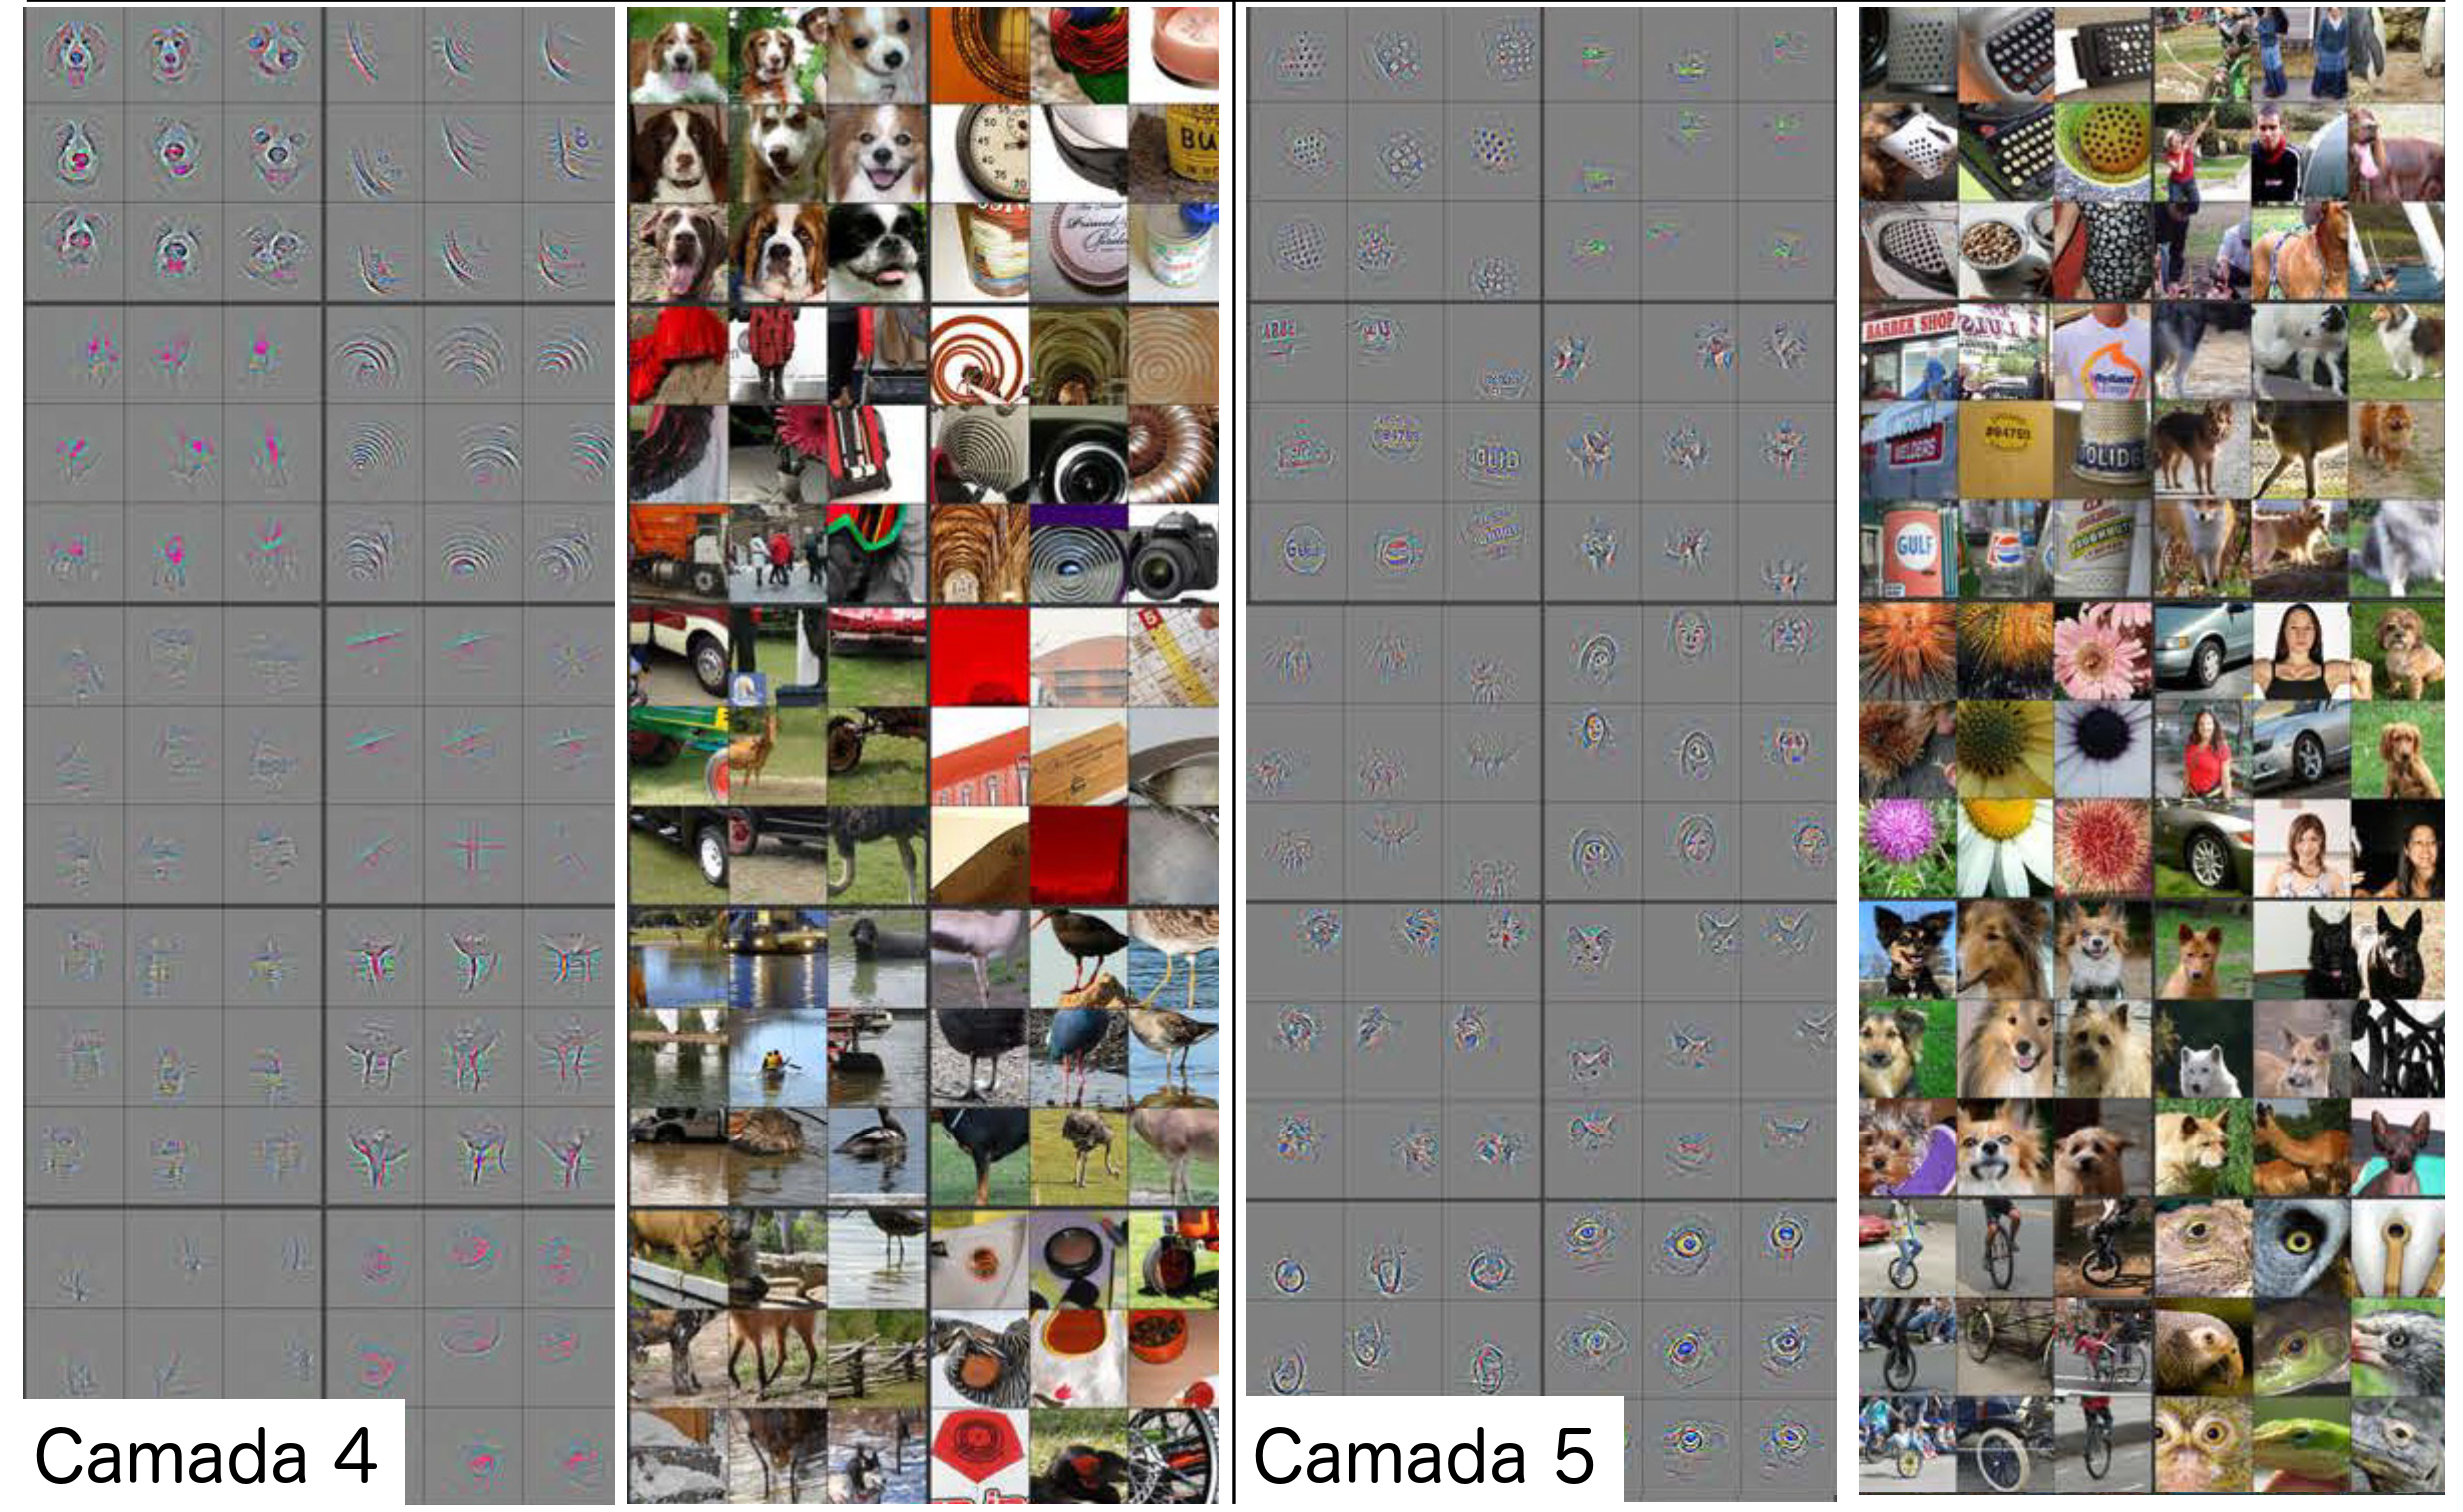
\includegraphics[width=0.95\linewidth]{{figuras/feature-4-5.png}}
  \caption{Quarta e quinta camada. \\ Fonte: \cite{Zeiler2013}}
 \end{center}
\end{figure}
\end{frame}

%-----------------------------------------------------------------------------
\subsection{Máquina de Boltzmann restrita}
\begin{frame}{Máquina de Boltzmann restrita}
\setlength\leftmargini{0em}
\justifying
 \begin{figure}[hbpt]
 \begin{center}
   \includegraphics[width=.5\linewidth]{{figuras/rbm.png}}
 \end{center}
  % \caption{Quarta e quinta camada. \\ Fonte: \cite{Zeiler2013}}
\end{figure}
\begin{itemize}
  \item Rede neural estocástica que treina um modelo a partir dos vetores de entrada;
  \item Os pixels correspondem às unidades visíveis e os detectores de características às unidades ocultas;
  \item Começa em um estado aleatório e atualiza seus pesos até encontrar uma distribuição que esteja em equilíbrio;
\end{itemize}

\end{frame}

\begin{frame}{Máquina de Boltzmann restrita}
\setlength\leftmargini{0em}
\justifying
\setstretch{1.2}
\begin{itemize}
  \item Identificar se uma imagem é relevante para o aprendizado.
\end{itemize}

\end{frame}

%-----------------------------------------------------------------------------
\subsection{Desbalanceamento de classes}
\begin{frame}{Desbalanceamento de classes}
\setlength\leftmargini{0em}
\justifying
\setstretch{1.2}
\begin{itemize}
  \item Número desbalanceado de exemplos. Majoritárias x minoritárias.
  \item Abordagens
    \begin{itemize}
        \item Reamostrar os dados;
        \item Adicionar funções de custo na classificação.
    \end{itemize}
\end{itemize}

% O desbalanceamento de classes é identificado quando determinadas classes possuem um número muito maior de elementos do que outras. Em conjuntos de dados desbalanceados, as classes com mais elementos são chamadas de classes majoritárias, e as com menos elementos, de minoritárias.

% \citet{Castro2011} destacam que duas abordagens têm sido utilizadas para solucionar esse problema: pode-se utilizar o pré-processamento dos dados de forma a rebalancear as distribuições das classes ao reamostrar os dados; ou então modificar métodos de aprendizado, como adicionar funções de custo na classificação. Esta pesquisa tem como enfoque o pré-processamento dos dados, ao rebalancear as classes através da geração de imagens artificiais.

\end{frame}
%-----------------------------------------------------------------------------
\begin{frame}{Desbalanceamento de classes - Sobreamostragem}
\setlength\leftmargini{0em}
\justifying
    \begin{itemize}
        \item Aumentar o número de elementos do conjunto;
        \item Replicação não reporta melhorias;
    \begin{block}{SMOTE}
    \justifying
\setlength\leftmargini{1em}
        \begin{itemize}
            \item Multiplica a diferença entre o vetor de características de um elemento e do seu vizinho mais próximo por um número [0-1];
            \item Adiciona ao vetor original, criando um novo elemento entre os dois vetores originais;
            \item Aprendida como exemplo da classe minoritária;
            \item Força uma região de decisão maior e mais geral;
        \end{itemize}
    \end{block}
    \end{itemize}



% Realizar uma sobreamostragem em um determinado conjunto de dados significa aumentar, utilizando alguma estratégia, o número de elementos desse conjunto. Em \citet{Chawla2002}, a simples replicação de exemplos já existentes na classe minoritária não melhorou a classificação. Isso se deve ao reconhecimento de regiões muito específicas, causando \textit{overfitting}.

% O SMOTE é uma técnica para rebalancear classes ao gerar artificialmente novos elementos, ao invés de apenas replicá-los. É aplicado sobre os vetores de características previamente extraídos, com operações de perturbação dos dados de treino (como rotação, por exemplo) no espaço de características, e não no espaço dos dados. A diferença entre o vetor de características de um elemento e do seu vizinho mais próximo é multiplicada por um número aleatório entre zero e um. Esse valor é adicionado ao vetor original, criando um novo elemento. Essa abordagem provoca a geração de um elemento entre os dois vetores originais. Os exemplos sintéticos forçam uma região de decisão maior e mais geral para serem aprendidas como exemplos da classe minoritária \cite{Chawla2002}.

% Dessa forma, o SMOTE provê mais elementos para o classificador aprender, ao contrário da replicação de dados. Como trabalhos futuros, \citet{Chawla2002} apontam que diferentes estratégias para criar esses exemplos sintéticos podem melhorar a performance da classificação. Inclusive salientando exemplos que foram errôneamente classificados.

% Uma variação desse algoritmo, denominada Borderline-SMOTE1 \cite{Han2005}, considera que elementos fora da linha de borda de cada classe pouco contribuem para a classificação. Por isso, propôe a geração de elementos sintéticos utilizando apenas elementos de borda. Considera que se os vizinhos mais próximos são da classe majoritária, o exemplo é ruído, e se há mais vizinhos da classe majoritária do que da minoritária, considera esse elemento como sendo de borda. Como trabalho futuro, destacam a necessidade de considerar diferentes estratégias para definir em quais elementos realizar o over-sampling.
\end{frame}
%-----------------------------------------------------------------------------
\begin{frame}{Contextualização - SMOTE}
\setlength\leftmargini{0em}
\justifying
 \begin{figure}[hbpt]
 \begin{center}
   \includegraphics[width=.6\linewidth]{{figuras/smote.jpeg}}
   % http://www.intechopen.com/books/advances-in-data-mining-knowledge-discovery-and-applications/selecting-representative-data-sets
 \end{center}
\end{figure}
\justifying
    \begin{itemize}
        \item Rebalancear classes ao gerar artificialmente novos elementos, ao invés de apenas replicá-los;
        \item Sobre os vetores de características previamente extraídos;
        \item (Chawla et al., 2002) \textbf{Diferentes estratégias para criar exemplos sintéticos podem melhorar a performance da classificação.}
    \end{itemize}
\end{frame}
%-----------------------------------------------------------------------------
\begin{frame}{Desbalanceamento de classes - Subamostragem}
\setlength\leftmargini{0em}
\justifying
    \begin{itemize}
        \item Diminuir o número de elementos do conjunto;
        \item Eliminar elementos da classe majoritária distantes da fronteira de decisão;
        \item Normalmente apresentam resultados piores;
        \item Podem remover informações essenciais dos dados originais;
        \item Não há melhor para todos os cenários.
    \end{itemize}
% Ao contrário da sobreamostragem, a subamostragem visa diminuir o número de elementos de um determinado conjunto. A ideia é eliminar elementos da classe majoritária que estão distantes da fronteira de decisão, isso porque eles são considerados menos relevantes para a aprendizagem.

% Métodos para remoção de exemplos da classe majoritária normalmente apresentam resultados piores do que métodos de sobreamostragem, conforme relatado por \citet{Batista2004} e \cite{Japkowicz2002}. Um dos motivos pela preferência natural a sobreamostragem é o fato de que ao realizar subamostragem pode-se remover informações essenciais dos dados originais. Mas não há uma estratégia única que funcione melhor para todos os cenários.
\end{frame}
%%%%%%%%%%%%%%%%%%%%%%%%%%%%%%%%%%%%%%%%%%%%%%%%%%%%%%%%%%%%%%%%%%%%%%%%%%%%%%%
\section{Proposta}
\begin{frame}{Metodologia}
\setstretch{1.2}
\setlength\leftmargini{1em}
\begin{block}{Características latentes}
\justifying
\begin{itemize}
\item Métodos de pré-processamento de imagens com o objetivo de obter imagens processadas que sejam melhor caracterizadas para a etapa de classificação. 
\item O enfoque em realçar determinadas características, utilizando diversos algoritmos sobre as imagens originais.
\end{itemize}
\end{block}
\end{frame}
%-----------------------------------------------------------------------------
\begin{frame}{Metodologia}
\setstretch{1.2}
\setlength\leftmargini{1em}
\begin{block}{Redes neurais}
\justifying
\begin{itemize}
\item Estado da arte da classificação, reconhecimento e localização de objetos;
\item Identificar as características relevantes em imagens;
\item RBM são redes neurais mais simples, convenientes para a verificação da relevância de uma imagem para o aprendizado.
\end{itemize}
\end{block}
\begin{block}{Desbalanceamento de classes}
\justifying
% esse problema é fundamentado em reconhecimento de padrões, e consiste em lidar com um conjunto de classes que possuem quantidades desiguais de imagens. Deve-se assim 
Pesquisar métodos que visam equilibrar o número de imagens em cada classe.
\end{block}
\end{frame}
%-----------------------------------------------------------------------------
\begin{frame}{Metodologia}
\setstretch{1.2}
\setlength\leftmargini{1em}
\begin{block}{Descritores}
\justifying
Investigar métodos capazes de descrever as propriedades das imagens.
\end{block}
\begin{block}{Classificador de padrões}
\justifying
\begin{itemize}
\item Naive Bayes, Optimum-Path Forest, KNN (\textit{K-Nearest Neighbor}) e Support Vector Machines. %A depender da performance do sistema após experimentos um destes será escolhido
\item Não é o foco deste estudo, após experimentos um destes será escolhido.
\end{itemize}
\end{block}
\end{frame}
%-----------------------------------------------------------------------------
\begin{frame}{Metodologia}
\setstretch{1.2}
\setlength\leftmargini{1em}
\begin{block}{Implementação}
\justifying
\begin{itemize}
\item Biblioteca OpenCV; %\cite{Intel2010}. 
\item Linguagens de programação C++ e Python;
\item Código disponível em \footnotesize{\url{https://bitbucket.org/moacirponti/imagefeatureextraction/overview}}. 
\end{itemize}
\end{block}
\end{frame}
%-----------------------------------------------------------------------------
\begin{frame}{Metodologia}
\setstretch{1.2}
\setlength\leftmargini{1em}
\begin{block}{Bases de imagens}
\justifying

\begin{itemize}
\item Objetivos com viés genérico;
\item Diversas coleções de imagens com o objetivo de estabelecer ou refutar as hipóteses levantadas;
\item Resultados preliminares com a base de imagens COREL\footnote{Disponível em http://wang.ist.psu.edu/docs/related/};
\end{itemize}
\end{block}
 
 % composta por fotografias que representam as classes: tribos africanas, praia, construções, ônibus, dinossauros, elefantes, flores, cavalos, montanhas e tipos de comidas. São 10 classes balanceadas com 100 imagens cada. Para fins de exemplificação, foram selecionadas imagens que representam essas classes na Figura \ref{fig:corel}. 
 
 \begin{figure}[hbpt]
 \begin{center}
   \includegraphics[width=0.8\linewidth]{\detokenize {figuras/exemplos_corel.png}}
 \end{center}
  \caption{Base de imagens COREL-1000}
\end{figure}
\end{frame}
%-----------------------------------------------------------------------------
\begin{frame}{Metodologia}
\setstretch{1.2}
\setlength\leftmargini{1em}
\begin{block}{Bases de imagens}
\justifying
\begin{itemize}
\item Cor: COREL-1000;
\item Textura: Describable Textures Dataset\footnote{http://www.robots.ox.ac.uk/~vgg/data/dtd/} (DTD);
\item Forma: Leafsnap\footnote{http://leafsnap.com/dataset/};
\end{itemize}
\end{block}
\vspace{1em}
\begin{columns}
  \begin{column}{0.5\textwidth}
    \begin{figure}[hbpt]
      \begin{center}
        \includegraphics[width=\columnwidth]{figuras/leafs.png}
      \end{center}
      \caption{Base de imagens Leafsnap.}
    \end{figure}
    \end{column}
  \begin{column}{0.5\textwidth}
    \begin{figure}[hbpt]
      \begin{center}    
        \includegraphics[width=\columnwidth]{figuras/texture.png}
       \end{center}
      \caption{Base de imagens DTD.}
    \end{figure}
  \end{column}
\end{columns}
\end{frame}
%-----------------------------------------------------------------------------
\begin{frame}{Metodologia}
\setstretch{1.2}
\setlength\leftmargini{1em}
\begin{block}{Experimentos}
\justifying
\begin{itemize}
\item Experimentos direcionados a explorar as etapas de pré-processamento, para melhorar a acurácia da classificação de bases de imagens;
\item Entrada: imagens originais provenientes de diversas coleções disponíveis na literatura;
\item Resultado: medidas estatísticas da classificação após a alteração das imagens com os métodos de realce de características relevantes.
\end{itemize}
\end{block}
\end{frame}
%----------------------------------------------------------------------------- 
\begin{frame}{Metodologia}
\setstretch{1.2}
\setlength\leftmargini{1em}
\begin{block}{Análise dos dados}
\justifying
\begin{itemize}
\item Comparar a classificação das imagens originais com aquelas tratadas pelo método proposto;
\item Ainda, o método de rebalanceamento de classes será comparado com técnicas disponíveis na literatura, como o SMOTE.
\end{itemize}
\end{block}
\end{frame}
% a medida estatística mais comum para avaliação é a razão do número de acertos pela quantidade de imagens testadas. Essa medida, conhecida por \underline{acurácia}, pode não refletir propriamente os resultados, em um cenário de bases desbalanceadas. Isso se deve ao fato de que se a classe minoritária não obtiver nenhum resultado correto e a classe majoritária tiver 100\% de acertos, a acurária normal poderá ser muito alta, mesmo considerando que nenhuma imagem da classe minoritária foi corretamente classificada. Dessa forma, considera que os erros são igualmente importantes. Mas em se tratando de bases desbalanceadas, deve-se diferenciar o erro em, por exemplo, diagnosticar um paciente doente -- classe minoritária -- como sendo saudável e um paciente saudável -- classe majoritária -- como estando doente \cite{Batista2004}. No primeiro caso, o paciente corre risco de diagnóstico tardil, enquanto o paciente saudável realiza outros testes para refutação.

% Pode-se estender essa medida obtendo-se a \underline{acurácia $k$-fold}: medida de acerto baseada na divisão do conjunto de objetos em teste e treinamento, realizando a repetição dos experimentos $n$ vezes e obtendo a média e o desvio padrão. A acurácia de cada experimento é obtida pela Equação~\ref{eq:Accuracy}, que considera problemas de desbalanceamento de classes.
%-----------------------------------------------------------------------------
\begin{frame}{Metodologia}
\setstretch{1.2}
\setlength\leftmargini{1em}
\begin{block}{Avaliação - F1Score}
\justifying
Efetividade da classificação em cenários desbalanceados. 
% Pode efetivamente avaliar a performance de classificação em cenários desbalanceados. 
\begin{itemize}

\item Precisão (exatidão): dos exemplos classificados como positivos, quantos realmente são.
\only<1>{
\begin{equation*}
  P = \frac{VP}{VP + FP}
\end{equation*}
}

\item Revocação (completude): quantos exemplos positivos foram corretamente classificados como tal. 
\only<1>{
\begin{equation*}
  R = \frac{VP}{VP + FN}
\end{equation*}
}
\end{itemize}

\only<2>{
\begin{equation*}
  F1 = 2 \frac{PR}{P+R}
\end{equation*}
}
\end{block}
\end{frame}
%-----------------------------------------------------------------------------
% Uma outra medida para bases desbalanceadas é a \underline{medida-F1} (conhecida como \textit{F1-Measure} ou \textit{F1-Score} e apresentada na Equação~\eqref{medidaf}), que combina precisão e revocação como medida de 
% A partir dessas medidas, o \underline{teste estatístico de Friedman} pode ser usado para determinar se há diferença significante em uma amostra de resultados gerados \cite{friedman2010}. As performances dos algoritmos são analisados e um \textit{rank} é atribuído para cada conjunto de dados. Ele considera que a hipótese nula a ser testada é que não há diferença estatística relevante entre as observações. Para analisar se o teste da hipótese é significativo, pode ser utilizado o \underline{p-valor}, que indica o quão estatisticamente significante o resultado é: quanto menor o seu valor, maior a evidência contra a hipótese nula (geralmente o limiar utilizado é de 0,05).

\begin{frame}{Metodologia}
\setstretch{1.2}
\setlength\leftmargini{1em}
\begin{block}{Avaliação - Friedman}
\begin{itemize}
\item Determinar se há diferença significante em uma amostra de resultados gerados;
\item As performances dos algoritmos são analisados e um \textit{rank} é atribuído para cada conjunto de dados;
\item A hipótese nula a ser testada é que não há diferença estatística relevante entre as observações;
\item P-valor indica o quão estatisticamente significante o resultado é: quanto menor o seu valor, maior a evidência contra a hipótese nula (limiar de 0,05).
\end{itemize}
\end{block}
\end{frame}
%-----------------------------------------------------------------------------
\begin{frame}{}
\setstretch{1.2}
\setlength\leftmargini{1em}
\begin{block}{Avaliação - Mahalanobis}  %\cite{mahalanobis2000}
Distância entre a média das classes e a variância dentro das classes. Baseia na correlação entre as variáveis e pode ser definida por
\begin{equation*}
  D_m(x_i) = \sqrt{(x_i - \mu)C^{-1}(x_i-\mu)^T},
\end{equation*}
\noindent onde $x_i$ é um vetor de valores, $\mu$ a média e C a matriz de covariância.
\end{block}
\end{frame}
%-----------------------------------------------------------------------------
\subsection{Resultados esperados}
\begin{frame}{Resultados Esperados}
\setlength\leftmargini{0em}

\begin{itemize}
\item \textit{Pré-processamento} de imagens que caracterizem melhor aspectos de suas classes, aumentando a variância entre as classes quando comparado com as imagens originais.
\item \textit{Geração artificial de imagens} de classes minoritárias de forma a compensar o desbalanceamento natural das bases de dados.
\item Melhorar a classificação, validando-a com a medida-F1. 
\item Análise as características aprendidas com o treinamento de uma CNN com bases específicas que destaquem propriedades como cor, textura e forma. 
\item Escolher imagens que adicionam informação ao conjunto de treino (RBM).
\item Bases naturalmente não balanceadas serão testadas e seus resultados avaliados.
\end{itemize}

% Os resultados esperados são relacionados às áreas de \textbf{processamento de imagens e reconhecimento de padrões}. Espera-se obter uma comprovação das hipóteses levantadas por essa pesquisa. Os resultados são esperados em duas vertentes:

% \begin{enumerate}
%  \item \textit{Pré-processamento} de imagens que caracterizem melhor aspectos de suas classes, aumentando a variância entre as classes quando comparado com as imagens originais.
%  \item \textit{Geração artificial de imagens} de classes minoritárias de forma a compensar o desbalanceamento natural das bases de dados.
% \end{enumerate}

% Em ambos os casos pretende-se melhorar a classificação, validando-a através do cálculo da medida-F1. A análise das características aprendidas por uma rede neural de convolução será realizada ao executar o treinamento com bases específicas que destaquem propriedades como cor, textura e forma. Além disso, os resultados serão obtidos a partir da escolha de quais imagens adicionam informação ao conjunto de treino. As redes RBM serão utilizadas para este fim. Bases naturalmente não balanceadas serão testadas e seus resultados avaliados.

\end{frame}
%-----------------------------------------------------------------------------
\subsection{Atividades e cronograma}
\begin{frame}{Atividades e Cronograma}
\definecolor{cinza}{rgb}{0.5,0.5,0.5}
\newcommand{\y}{\color{black}\rule{20pt}{7pt}}
\newcommand{\x}{\hspace*{20pt}}
\renewcommand{\r}{\color{cinza}\rule{20pt}{7pt}}
% \setlength{\tabcolsep}{0pt}
\begin{table}
\caption{Duração de cada atividade a partir de 24/02/2014.}
\begin{center}
\begin{tabular}{|c|c|c|c|c|c|}
 \cline{2-6}
\multicolumn{1}{l|}{} & \multicolumn{2}{c|}{2014} & \multicolumn{2}{c|}{2015} & 2016 \\
\hline \ Atividade\ \ & 1\textordmasculine\ Sem. & 2\textordmasculine\
Sem. & 1\textordmasculine\ Sem. & 2\textordmasculine\ Sem. & 1\textordmasculine\ Sem. \\
\hline \hline
%   &         2014        &       2015         \\
1   &\y\y    &\y\y      &\x\x     &\x\x    &\x \\
\hline
2   &\x\x    &\y\y      &\r\r     &\x\x    &\x \\
\hline
3   &\x\x    &\y\y      &\r\r     &\r\x    &\x \\
\hline
4   &\x\x    &\x\x      &\x\r     &\r\r    &\x \\
\hline
5   &\x\x    &\x\y      &\r\r     &\r\r    &\x \\
\hline
6   &\x\x    &\x\y      &\r\x     &\x\r    &\r\x  \\
\hline
\end{tabular}
\end{center}
\end{table}
\end{frame}
%%%%%%%%%%%%%%%%%%%%%%%%%%%%%%%%%%%%%%%%%%%%%%%%%%%%%%%%%%%%%%%%%%%%%%%%%%%%%%%
\section{Resultados Preliminares}
\begin{frame}{Resultados Preliminares}
\setlength\leftmargini{1em}
\renewcommand{\tabcolsep}{0.04cm}
\begin{figure}[!h]
 \begin{center}
 \begin{tabular}{ccccc}
   \includegraphics[width=0.245\linewidth]{\detokenize {figuras/original-1.jpg}}&
   \includegraphics[width=0.245\linewidth]{\detokenize {figuras/original-2.jpg}}&
   \includegraphics[width=0.245\linewidth]{\detokenize {figuras/original-3.jpg}}&
   % \includegraphics[width=0.19\linewidth]{\detokenize {figuras/original-4.jpg}}&
   \includegraphics[width=0.245\linewidth]{\detokenize {figuras/original-5.jpg}}\\
   \includegraphics[width=0.245\linewidth]{\detokenize {figuras/gerada-1_blur.jpg}}&
   \includegraphics[width=0.245\linewidth]{\detokenize {figuras/gerada-2_ruido.jpg}}&
   \includegraphics[width=0.245\linewidth]{\detokenize {figuras/gerada-3_blend.jpg}}&
   % \includegraphics[width=0.19\linewidth]{\detokenize {figuras/gerada-4_unsharpMask.jpg}}&
   \includegraphics[width=0.245\linewidth]{\detokenize {figuras/gerada-5.jpg}} \\
 \end{tabular}
 \end{center}
  \caption{Geração de imagens artificiais para o rebalanceamento de classes por meio de: borramento, adição de ruído, mistura e combinação.}
\end{figure}
\renewcommand{\tabcolsep}{0.5cm}
\vspace{25pt}
\end{frame}
%-----------------------------------------------------------------------------
% Os descritores de características utilizados para os resultados foram apresentados na Seção \ref{sec:extracao}. Considerando que em um experimento anterior o melhor resultado foi atribuído à quantização com o método de Intensidade para o extrator Haralick e MSB para os outros, apenas esses testes foram aprofundados (tópico anteriormente discutido na Seção \ref{sec:quantizacao}). Neste experimento o classificador KNN foi utilizado, com $K=1$. Inicialmente o classificador Naive Bayes foi explorado, apresentando melhora na acurácia ao apenas replicar as imagens. Esse comportamento não é desejado em um classificador para a avaliação de rebalanceamento de classes. O código desenvolvido para esses resultados preliminares está disponível em \url{https://bitbucket.org/moacirponti/imagefeatureextraction/overview}. 
\subsection{Descrição do experimento}
\begin{frame}[plain]{Descrição do Experimento}
\begin{figure}[!htb]
 \begin{center}
   \includegraphics[width=0.65\textheight]{\detokenize {figuras/flow_main.pdf}}
 \end{center}
  \caption{Fluxo dos resultados preliminares.}
\end{figure}
\end{frame}
%-----------------------------------------------------------------------------
\begin{frame}[plain]{Descrição do Experimento}
\begin{figure}[!htb]
 \begin{center}
   \includegraphics[width=0.6\textheight]{\detokenize {figuras/flow_sub.pdf}}
 \end{center}
  \caption{Fluxo da geração artificial.}
\end{figure}
\end{frame}
%-----------------------------------------------------------------------------
\subsection{Resultados}
\begin{frame}{Resultados Preliminares}
\setlength\leftmargini{0em}
\setstretch{1.2}
\justifying
Classes com maior dificultade de diferenciação, havendo alta taxa de sobreposição de intensidades de cores e texturas.
\begin{figure}[!htb]
 \begin{center}
   \includegraphics[width=\linewidth]{\detokenize {figuras/praia-montanha.png}}
 \end{center}
  \caption{Classes ``praia'' e ``montanha'' da base de imagens COREL-1000.}
\end{figure}
\end{frame}
%-----------------------------------------------------------------------------
\begin{frame}{Resultados Preliminares - Melhor}
\setlength\leftmargini{0em}
\justifying
\begin{itemize}
\item Ganho estatístico da medida-F, quando comparado à geração de exemplos artificiais no espaço de atributos; % (ou seja, depois que as características já foram extraídas das imagens)
% \item Descritor ACC, conversão MSB e operação de pré-processamento combinação. 
\end{itemize}
\vspace{-0.3cm}
\begin{figure}[htb]
 \begin{center}
   \includegraphics[width=0.7\linewidth]{\detokenize {figuras/resultado-melhor4.png}}
 \end{center}
 \caption{Resultado obtido com a operação de combinação.}
\end{figure}
\end{frame}
%-----------------------------------------------------------------------------
\begin{frame}{Resultados Preliminares - Pior}
\setlength\leftmargini{0em}
\setstretch{1.2}
\justifying
\begin{figure}[htb]
 \begin{center}
   \includegraphics[width=0.8\linewidth]{\detokenize {figuras/resultado-pior1.png}}
 \end{center}
 \caption{Piores resultados, obtidos com a adição de ruído.}
\end{figure}
% \begin{itemize}
% % \item Adição de ruído, extração com CCV e a quantização por MSB;
% \end{itemize}
\end{frame}
%-----------------------------------------------------------------------------
\begin{frame}{Resultados Preliminares}
\setlength\leftmargini{0em}
\setstretch{1.2}
\justifying
\begin{itemize}
\item Melhores operações: todas, apenas mistura e apenas composição;
\item Piores: apenas borramento, ruído ou \textit{unsharp masking};
\vspace{2pt}
\item Melhor extrator: ACC;
\item Piores: CCV e GCH;
% \vspace{2pt}
% \item Melhor quantizador: MSB;
% \item Piores: CCV e GCH;
\end{itemize}
\end{frame}
%-----------------------------------------------------------------------------
\begin{frame}{Resultados Preliminares}
\setlength\leftmargini{0em}
\setstretch{1.2}
\justifying
\begin{itemize}
\item Teste de Friedman para todas as execuções das melhores operações. 
\item P-valor = $4.24E^{-11}$. Hipótese nula rejeitada;
\end{itemize}
\begin{table}[htb]
\centering
\caption{Posição média dos algoritmos utilizando Friedman}
  \begin{tabular}{c|c}
    Algoritmos  &   Posição \\ \hline
    Original    &   3.0000  \\
    Smote       &   1.6136  \\
    Artificial  &   1.3863  \\
  \end{tabular}
\end{table}
\begin{itemize}
\item Em algumas execuções: geração artificial (1), SMOTE (2) e imagens originais (3).
\end{itemize}
\end{frame}
%-----------------------------------------------------------------------------
\begin{frame}{Resultados Preliminares}
\setlength\leftmargini{0em}
\setstretch{1.2}
\justifying

\begin{itemize}
\item Replicação: SRS - \textit{Simple Random Sampling};
\item Não adiciona informações novas para o aprendizado.
\end{itemize}

\begin{figure}[htb]
 \begin{center}
   \includegraphics[width=0.7\linewidth]{\detokenize {figuras/resultado-copia.png}}
 \end{center}
  \caption{Simples replicação de exemplos sem realizar nenhuma operação de pré-processamento.}
\end{figure}
\end{frame}
%%%%%%%%%%%%%%%%%%%%%%%%%%%%%%%%%%%%%%%%%%%%%%%%%%%%%%%%%%%%%%%%%%%%%%%%%%%%%%%
\begin{frame}{Resultados Preliminares - CNN}
\begin{table}
\caption{CNN para classes praia e montanha da base COREL-1000.}
  \begin{tabular}{c|c}
    Algoritmos    &   Medida F1 \\ \hline
    Original      &   0.708  \\
    Desbalanceada &   0.577  \\
    Rebalanceada  &   0.677  \\
  \end{tabular}
\end{table}
\end{frame}
%%%%%%%%%%%%%%%%%%%%%%%%%%%%%%%%%%%%%%%%%%%%%%%%%%%%%%%%%%%%%%%%%%%%%%%%%%%%%%%
\subsection{Artigo}
\begin{frame}{Artigo na Neurocomputing}
\setstretch{1.5}
\begin{block}{}
\justifying
Ponti, M.; Nazaré, T; Thumé, G. \textbf{Image quantization as a dimensionality reduction procedure in color and texture feature extraction}, submitted to Neurocomputing, 2014.
\end{block}
\end{frame}
%%%%%%%%%%%%%%%%%%%%%%%%%%%%%%%%%%%%%%%%%%%%%%%%%%%%%%%%%%%%%%%%%%%%%%%%%%%%%%%
\section{Próximos Passos}
\setlength\leftmargini{0em}
\setstretch{1.2}
\justifying
\begin{frame}{Próximos Passos}
  \begin{itemize}
  \item Analisar as características latentes que as redes neurais de convolução conseguem extrair
    \begin{itemize}
      \item Bases bem discriminadas quanto às propriedades de textura, cor e forma.
    \end{itemize}
  \item Analisar a memória associativa de uma rede de Boltzmann 
  \begin{itemize}
    \item As imagens geradas foram adicionadas no conjunto de treino sem verificação da sua relevância;
    \item Escolha para qual imagem original utilizar, ao invés do método aleatório utilizado nos resultados preliminares.
  \end{itemize}
  \end{itemize}

% O treinamento de uma rede neural de convolução~\footnote{\url{http://caffe.berkeleyvision.org/}} foi realizado, utilizando as classes ``praia'' e ``montanha'', balanceadas, da base COREL-1000. A classificação desse treinamento obteve $\approx 80\%$ de acurácia, enquanto que utilizando os extratores padrões foi possível atingir apenas $\approx 69\%$. Isso reforça a proposta de analisar quais são as características latentes que esse tipo de rede neural consegue extrair. Para essa análise vão ser utilizadas bases discriminadas quanto às propriedades de textura, cor e forma.

% Além de analisar o processamento realizado por uma rede de convolução para a classificação das imagens, uma rede RBM também será treinada para análise da sua memória associativa. As imagens artificialmente geradas foram adicionadas no conjunto de treino sem verificação da sua relevância, o que pode ter prejudicado a classificação. A memória associativa aprendida com o treinamento de uma máquina de Bolztmann restrita pode vir a auxiliar no entendimento dessas imagens como relevantes ou não. Além disso, pode servir como escolha para qual imagem original utilizar, ao invés do método aleatório utilizado nos resultados preliminares.

\end{frame}
%-----------------------------------------------------------------------------
\begin{frame}{Próximos Passos}
\setlength\leftmargini{0em}
\setstretch{1.2}
\justifying
  \begin{itemize}
  \item Desbalancear as 10 classes da COREL-1000 em escada;
  \item Utilizar todas as classes com apenas 1 desbalanceada;
  \item Analisar o treinamento da CNN para as 3 bases bem discriminadas.
  \end{itemize}
\end{frame}
%-----------------------------------------------------------------------------
\begin{frame}{Agradecimentos}
\begin{columns}
  \begin{column}{0.5\textwidth}
  \centering
    \includegraphics[width=0.6\columnwidth]{figuras/cnpqLogo.jpg}
  \end{column}
  \begin{column}{0.5\textwidth}
  \centering
    \includegraphics[width=0.6\columnwidth]{figuras/brasao_usp_pb}
  \end{column}
\end{columns}
\end{frame}
%-----------------------------------------------------------------------------
\section{Referências}
\begin{frame}{Referências}
\end{frame}
%-----------------------------------------------------------------------------
\begin{frame}[plain]
  \maketitle
\end{frame}
%%%%%%%%%%%%%%%%%%%%%%%%%%%%%%%%%%%%%%%%%%%%%%%%%%%%%%%%%%%%%%%%%%%%%%%%%%%%%%%%
\end{document}
